\capitulo{4}{Metodología}

\section{Descripción de los datos.}
En este trabajo, las 34 ecografías proporcionadas por el Servicio de Ginecología y Obstetricia del Hospital Universitario de Burgos (HUBU) han servido como base para entrenar las distintas arquitecturas. Los datos fueron divididos en tres subconjuntos: entrenamiento, validación y prueba, con el fin de garantizar una evaluación sólida y evitar el sobreajuste del modelo. En este apartado se describen los datos utilizados.
 
\section{Técnicas y herramientas.}
\subsection{Entornos de desarrollo}
\subsubsection{Google Colab}
Google Colab\footnote{Sitio Web de Google Colab: \url{https://cloud.google.com/colab/docs?hl=es-419}} es una plataforma basada en la nube que permite ejecutar notebooks de Jupyter sin necesidad de configuración local. Está especialmente orientada a tareas de ciencia de datos, aprendizaje automático y educación, y ofrece acceso a recursos computacionales como GPUs y TPUs sin coste adicional. 

Los notebooks se almacenan directamente en Google Drive, lo que facilita el acceso desde cualquier lugar y permite la colaboración en tiempo real.
La plataforma es compatible con bibliotecas populares como PyTorch, TensorFlow, pandas y matplotlib, sin necesidad de instalaciones manuales. Permite ejecutar código Python, comandos del sistema e interactuar con el entorno como si fuera local, gracias a máquinas virtuales asignadas automáticamente. Su integración con el ecosistema de Google y su facilidad de uso la convierten en una herramienta ideal para prototipado de modelos de IA.
\subsubsection{Visual Studio Code}
Visual Studio Code \footnote{Sitio Web de Visual Studio Code: \url{https://code.visualstudio.com/}} (VS Code) es un editor de código fuente desarrollado por Microsoft, ampliamente utilizado por su ligereza, rapidez y capacidad de personalización mediante extensiones. En el presente proyecto, se ha utilizado como entorno principal para el desarrollo de la aplicación en Streamlit, permitiendo una edición fluida del código Python, así como la estructuración y prueba del flujo complementario de la herramienta.

Gracias a su integración con Git y GitHub, Visual Studio Code también ha facilitado la subida y gestión del proyecto en repositorios remotos, permitiendo un control de versiones eficiente y una organización clara del trabajo. 

\subsection{Streamlit}
Streamlit\footnote{Sitio Web de Streamlit: \url{https://streamlit.io/}} es un framework de código abierto en Python diseñado para crear aplicaciones web interactivas de forma rápida y sencilla. Su principal ventaja es que permite transformar scripts de Python en interfaces visuales accesibles a usuarios sin conocimientos técnicos.

En este proyecto, Streamlit ha sido utilizado para desarrollar una aplicación interactiva que permite ejecutar el modelo de segmentación sobre ecografías de cerebros fetales, visualizar los resultados de forma clara y descargar un informe en formato PDF con las predicciones generadas, con el fin de facilitar la documentación, el seguimiento clínico y la comunicación de resultados entre profesionales médicos.

Para facilitar su acceso y uso por parte de profesionales médicos o evaluadores externos, la aplicación ha sido desplegada en Streamlit Community Cloud\footnote{Sitio Web de Streamlit Community Cloud: \url{https://streamlit.io/cloud}}, la plataforma gratuita de alojamiento de aplicaciones desarrollada por los propios creadores de Streamlit. Esto ha permitido que la herramienta esté disponible en línea sin necesidad de configuración adicional por parte del usuario final.

\subsection{Lenguajes de programación}
\subsubsection{Python}
Python\footnote{Sitio Web de Python: \url{https://www.python.org/}} es un lenguaje de programación de propósito general, interpretado y de alto nivel, conocido por su sintaxis clara y legible. Esta característica facilita su aprendizaje, convirtiéndolo en una herramienta versátil aplicable en diversos ámbitos como el desarrollo web, la automatización, la ciencia de datos, la IA y el procesamiento de imágenes médicas.

Además, Python ofrece una extensa biblioteca estándar y un amplio ecosistema de paquetes de terceros. Es un lenguaje multiplataforma, de código abierto, respaldado por una comunidad global de desarrolladores que contribuyen de forma constante a su evolución.

En este proyecto, Python ha sido elegido como lenguaje principal debido a su flexibilidad, facilidad de uso y compatibilidad con bibliotecas especializadas en aprendizaje automático y procesamiento de imágenes médicas.
\subsubsection{LaTeX}
LaTeX\footnote{Sitio Web de LaTeX: \url{https://www.latex-project.org/}} es un sistema de preparación de documentos desarrollado sobre el lenguaje tipográfico TeX, orientado principalmente a la creación de textos técnicos y científicos. Su principal ventaja es que permite al autor centrarse en el contenido, mientras que el sistema se encarga automáticamente del formato y la presentación tipográfica.

Gracias a su enfoque basado en comandos estructurados, LaTeX facilita la gestión precisa de bibliografías, ecuaciones, referencias cruzadas, índices, tablas y figuras, ofreciendo resultados de alta calidad tipográfica. 

En el presente proyecto, se ha utilizado este sistema mediante el editor colaborativo Overleaf \footnote{Sitio Web de Overleaf: \url{https://es.overleaf.com/}}, lo que ha permitido una redacción eficiente y organizada del documento.
\subsection{Bibliotecas}
\subsubsection{Procesamiento de Datos y Manipulación de archivos}
\begin{itemize}
    \item \textbf{os} \footnote{Documentación de os: \url{https://docs.python.org/3/library/os.html}} y \textbf{shutil}\footnote{Documentación de shutil: \url{https://docs.python.org/3/library/shutil.html}}: son bibliotecas del módulo estándar de Python utilizadas para interactuar con el sistema de archivos. En este proyecto, \textbf{os} se ha utilizado para gestionar rutas y crea directorios de salida para almacenar resultados, mientras que \textbf{shutil} se ha empleado para mover imágenes entre carpetas, preservando la estructura del conjunto de datos durante el preprocesamiento.
    \item \textbf{pathlib.Path}\footnote{Documentación de pathlib: \url{https://docs.python.org/3/library/pathlib.html}}: \textbf{pathlib}, con su clase \textit{Path}, proporciona una interfaz orientada a objetos para la manipulación de rutas en el sistema de archivos. Se ha utilizado para crear, verificar y manipular rutas de entrada y salida de manera eficiente.
    \item \textbf{pandas}\footnote{Documentación de pandas: \url{https://pandas.pydata.org/docs/}}: es una biblioteca especializada en la manipulación y análisis de datos estructurados, proporcionando estructuras como DataFrame y Series. En este proyecto, se ha usado para organizar y procesar las métricas de evaluación de la segmentación, calcular medias de resultados y preparar las tablas de resultados que posteriormente se exportan como imágenes para su inclusión en los informes finales.
    \item \textbf{NumPy (Numerical Python)}\footnote{Documentación de NumPy: \url{https://numpy.org/doc/}}:es una biblioteca que ofrece estructuras de datos eficientes y un amplio conjunto de funciones para operaciones sobre arrays multidimensionales. En este proyecto, se ha empleado para convertir máscaras de segmentación en arrays numéricos, mapear colores RGB a clases enteras y ejecutar operaciones matriciales de manera rápida, como asignaciones, filtrado o conteo de clases. Esto es esencial para el preprocesamiento de datos y la preparación de entradas para el modelo de aprendizaje profundo.
\end{itemize}
\subsubsection{Procesamiento de imágenes}
\begin{itemize}
    \item \textbf{PIL}\footnote{Documentación de PIL: \url{https://pillow.readthedocs.io/en/stable/}}: a través de su versión moderna \textbf{Pillow}, es una biblioteca de procesamiento de imágenes que permite abrir, editar y guardar archivos de imagen. En el proyecto, se ha utilizado para generar máscaras segmentadas y convertirlas al formato necesario para el modelo.
    \item \textbf{cv2}\footnote{Documentación de OpenCV: \url{https://docs.opencv.org/4.x/index.html}}: correspondiente a OpenCv (Open Source Computer Vision Library), es una herramienta de visión por computador. Aquí se ha empleado para leer imágenes y máscaras, realizar conversiones de espacio de color (como RGB a escala de grises) y preparar los datos visuales para el modelo de segmentación.
\end{itemize}

\subsubsection{Modelado y entrenamiento}
\begin{itemize}
    \item \textbf{torch}\footnote{Documentación de torch: \url{https://docs.pytorch.org/docs/stable/index.html}}: es una biblioteca de código abierto especializada en la computación numérica basada en tensores. En el proyecto, ha servido como base para definir y entrenar el modelo de segmentación.
    \begin{itemize}
    \item \textbf{torch.utils.data}: proporciona herramientas para gestionar conjuntos de datos y facilitar la carga eficiente de datos durante el entrenamiento, organizándolos en batches y simplificando su acceso en cada época.
    \item \textbf{torch.optim.lr\_scheduler}: ofrece métodos para ajustar dinámicamente la tasa de aprendizaje durante el entrenamiento, optimizando la convergencia del modelo. Se ha utilizado para implementar estrategias de aprendizaje adaptativo y mejorar el rendimiento del modelo durante la segmentación.
    \end{itemize}
    \item \textbf{pytorch\_lightning}\footnote{Documentación de pytorch\_lightning: \url{https://lightning.ai/docs/pytorch/stable/}}: es un framework ligero y de alto nivel construido sobre PyTorch que organiza el código de entrenamiento de manera estructural y modular. En este trabajo, ha facilitado la definición de los flujos de entrenamiento, validación y prueba, reduciendo el código repetitivo y mejorando la reproducibilidad de los experimentos.
    \begin{itemize}
    \item \textbf{pytorch\_lightning.callbacks}: incluye herramientas automáticas para gestionar eventos durante el entrenamiento, como la parada temprana (\textit{Early Stopping}) y la monitorización del mejor modelo (\textit{Model Checkpoint}). Estas funciones optimizan el proceso de entrenamiento, asegurando un rendimiento eficiente.
    \end{itemize}
    \item \textbf{segmentation\_models\_pytorch}\footnote{Documentación de segmentation\_models\_pytorch}: \url{https://github.com/qubvel-org/segmentation_models.pytorch?tab=readme-ov-file#api}: es una biblioteca que proporciona implementaciones preentrenadas de modelos avanzados de segmentación de imágenes basados en PyTorch. En este proyecto, se ha utilizado para instanciar arquitecturas competitivas de segmentación, como U-Net++, acelerando el desarrollo y garantizando resultados de alta calidad.
\end{itemize}
\subsubsection{Evaluación y Métricas}
\begin{itemize}
    \item \textbf{scikit-learn}\footnote{Documentación de scikit-learn: \url{https://scikit-learn.org/stable/}}: es una biblioteca de aprendizaje automático que proporciona herramientas eficientes para análisis predictivo y modelado estadístico. En el proyecto se ha utilizado principalmente el siguiente módulo:
    \begin{itemize}
    \item \textbf{sklearn.model\_selection}: ofrece métodos para la división y validación cruzada de conjuntos de datos, optimizando la distribución de los datos en las fases de entrenamiento y evaluación.
    \end{itemize}
    \item \textbf{Matplotlib}\footnote{Documentación de Matplotlib: \url{https://matplotlib.org/stable/index.html}}: es una biblioteca especializada en la generación de gráficos y visualizaciones estáticas, animadas e interactivas. Se ha utilizado para representar resultados de segmentación y visualizar métricas de evaluación de forma gráfica.
    \begin{itemize}
    \item \textbf{matplotlib.pyplot}: proporciona una interfaz sencilla similar a MATLAB para la creación de gráficos. Se ha empleado para visualizar ejemplos de segmentaciones y evolución de métricas de entrenamiento.
    \item \textbf{matplotlib.colors.ListedColormap}: permite definir mapas de colores personalizados, utilizado para representar de forma diferenciada las distintas clases segmentadas en las predicciones del modelo.
    \end{itemize}
\end{itemize}

\subsubsection{Automatización de documentos}
\begin{itemize}
    \item \textbf{python-docx}\footnote{Documentación de python-docx: \url{https://python-docx.readthedocs.io/en/latest/}}: permite crear, modificar y exportar documentos en formato .docx (Microsoft Word) directamente desde Python. Se ha utilizado para automatizar la generación de informes finales, insertando tablas de métricas y resultados de la segmentación de manera estructurada.
\end{itemize}
\subsection{Preprocesamiento de datos}
\subsubsection{Roboflow}
Roboflow\footnote{Página Web de Roboflow: \url{https://docs.roboflow.com/}} es una plataforma integral para el desarrollo de modelos de visión por computador que permite gestionar, anotar, preprocesar y desplegar conjuntos de datos de imágenes. En el contexto del presente trabajo, Roboflow se ha utilizado principalmente para la creación de la \textit{ground truth}.

La herramienta permitió realizar anotaciones manuales mediante segmentación por instancias, utilizando polígonos para delimitar con precisión las estructuras cerebrales de interés. Esto facilitó la creación de máscaras detalladas, necesarias para entrenar modelos de segmentación con alta precisión. 

Además, ha permitido adaptar y modificar los conjuntos de datos según las necesidades del proyecto, ya sea combinando clases, reorganizando anotaciones o generando nuevas versiones conforme aumentaba su volumen. Gracias a sus funcionalidades de gestión y exportación flexible en formatos como COCO, se ha optimizado el flujo de trabajo de preparación de datos, facilitando su integración con entornos de desarrollo basados en PyTorch y PyTorch Lightning.

\subsubsection{Formato COCO}
El formato COCO (Common Objects in Context) es un estándar ampliamente utilizado en visión por computadora para estructurar anotaciones de imágenes en un archivo JSON. Este formato contiene toda la información necesaria para describir las imágenes y sus regiones segmentadas. Entre sus elementos clave se encuentran:
\begin{itemize}
    \item \texttt{categories}: contiene la lista de clases que se utilizan en el dataset. Están definidas con un \texttt{id} numérico y un \texttt{name}.
    \item \texttt{images}: describe las imágenes incluidas en el dataset. Contiene atributos como \textit{id}, \texttt{file\_name} (el nombre del archivo de imagen asociado) y \textit{height} y \texttt{width} (las dimensiones en píxeles de la imagen).
    \item \texttt{annotations}: anotaciones que especifican las regiones segmentadas. Contiene atributos como \texttt{bbox} (la caja delimitadora), \texttt{segmentation}(los puntos que delimitan la región segmentada) y \texttt{category\_id} (la categoría asociada). 
\end{itemize}
Este formato facilita la organización y procesamiento eficiente de datos en proyectos de visión por computadora.
    

\subsection{Herramientas software}
\subsubsection{GitHub}
GitHub\footnote{Página Web de GitHub: \url{https://docs.github.com/es}} es una plataforma de desarrollo colaborativo basada en Git, un sistema de control de versiones distribuido. Permite gestionar proyectos de software mediante repositorios, donde se almacenan, organizan y versionan los archivos. GitHub ha sido una herramienta clave para asegurar el desarrollo eficiente del proyecto, facilitando no solo la organización de tareas y el control de versiones a lo largo del proceso, sino también la creación del repositorio en línea, garantizando el respaldo y acceso remoto al código.
\section{Metodologías}
\subsection{CRISP-DM}
El desarrollo del presente proyecto se guiará por la metodología CRISP-DM (CRoss Industry Standard Process for Data Mining). Esta metodología proporciona un marco estructurado que permite planificar, gestionar y ejecutar proyectos de minería de datos de forma ágil y eficiente, asegurando la trazabilidad y validación en cada una de sus fases \cite{crispdm2021}.

CRISP-DM se compone de seis fases principales, que se desarrollarán de manera iterativa durante el proyecto:
\begin{itemize}
    \item \textbf{Comprensión del negocio (Business Understanding)}: En esta primera fase, se busca comprender en profundidad los objetivos del proyecto, definiendo criterios de éxito y evaluando los recursos disponibles.
    \item \textbf{Comprensión de los datos (Data Understanding)}: Se centra en identificar, recopilar u analizar los conjuntos de datos necesarios para alcanzar los objetivos del proyecto. 
    \item \textbf{Preparación de los datos (Data Preparation)}: Esta etapa incluye todas las tareas necesarias para dejar los datos listos para el modelado.
    \item \textbf{Modelado (Modeling)}: Se aplicarán técnicas de segmentación de imágenes, evaluando distintos algoritmos para determinar cuál ofrece mejores resultados en la detección de estructuras cerebelosas. 
    \item \textbf{Evaluación (Evaluation)}: Se evaluará el rendimiento de los resultados obtenidos para determinar si cumplen con los requisitos clínicos y científicos del proyecto.
    \item \textbf{Implementación (Deployment)}: Finalmente, el modelo será implementado en un entorno funcional, asegurando que sean accesibles y útiles para los interesados.
\end{itemize}
Cada una de estas fases incluirá tareas específicas con un cronograma de ejecución definido, permitiendo un desarrollo progresivo y controlado del proyecto hasta alcanzar los objetivos planteados \cite{crispdm2021}. La Figura \ref{fig:crispdm_diagrama} representa el flujo de trabajo de esta metodología.

\begin{figure}[h]
    \centering
    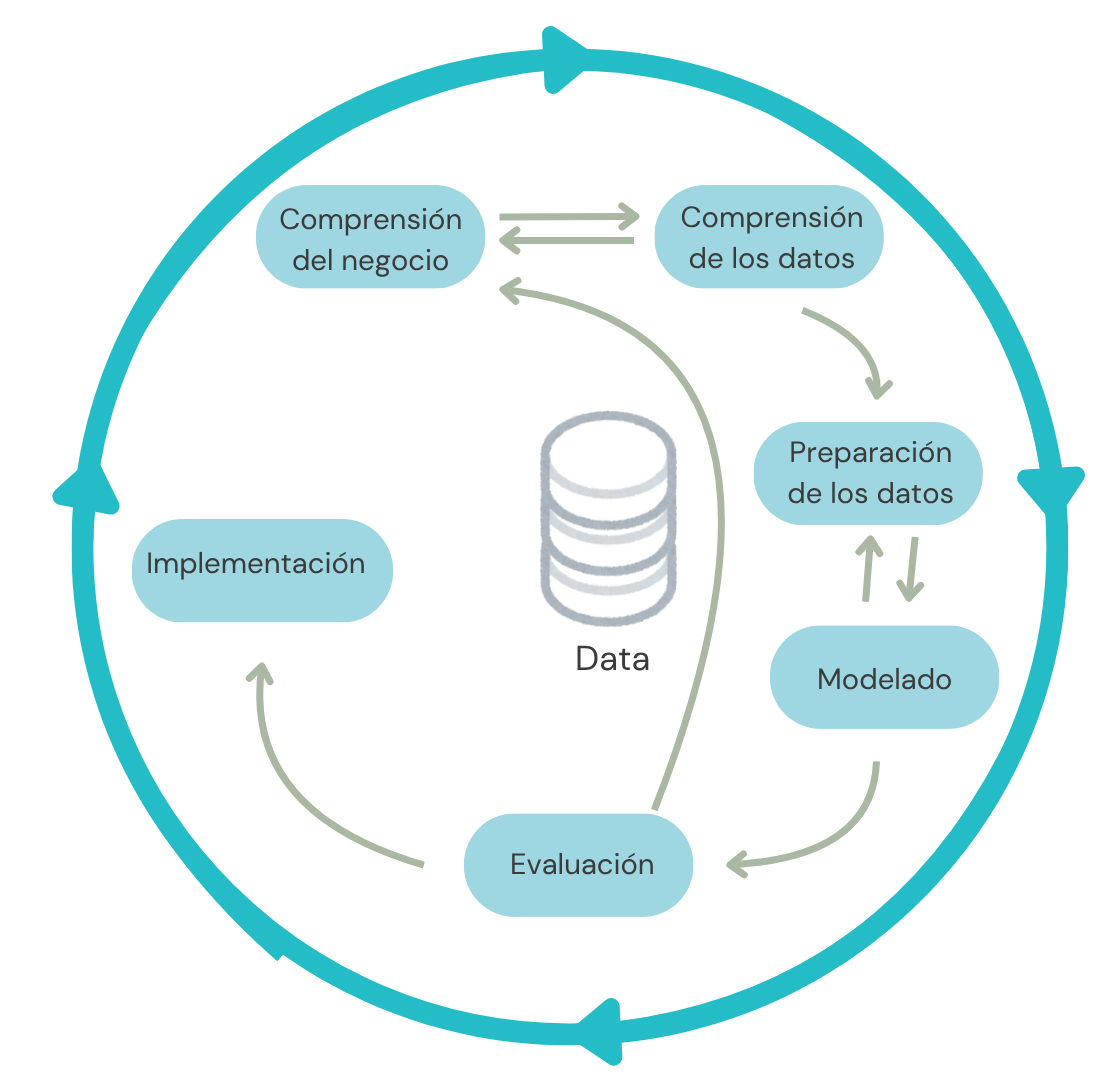
\includegraphics[width= 0.8\textwidth]{img/cripdm_flujo.png}
    \caption{Diagrama del proceso CRISP-DM, adaptado de \cite{crispdmimage}}
    \label{fig:crispdm_diagrama}
\end{figure}

\section{Técnicas}
\subsection{Hold-out}
Una de las técnicas usadas para garantizar que el modelo no solo aprende los datos del conjunto de entrenamiento, sino que también es capaz de generalizar a datos no vistos previamente es el método \textit{hold-out}. Esta consiste en dividir el conjunto de datos disponible en tres subconjuntos independientes \cite{deeplearning2016}:
\begin{itemize}
    \item \textbf{Conjunto de entrenamiento (\texttt{train})}: utilizado para ajustar los pesos internos del modelo. Durante esta fase, la red aprende los patrones presentes mediante el proceso de optimización y retropropagación del error (\textit{backpropagation}).
    \item \textbf{Conjunto de validación (\texttt{validation})}: empleado para evaluar el rendimiento del modelo durante el entrenamiento sin influir en el aprendizaje directo. Ayuda a ajustar \textit{hiperparametros} (como la tasa de aprendizaje o el número de capas) y detectar problemas como el \textit{sobreajuste} (\textit{overfitting}).
    \item \textbf{Conjunto de prueba (\texttt{test})}: permite medir el fin de su rendimiento final sobre datos completamente nuevos, y así obtener una estimación objetiva de su capacidad de generalización. 
\end{itemize}

\subsection{Sobreajuste}
El sobreajuste u \textit{overfitting} se produce cuando un modelo se ajusta excesivamente a los datos de entrenamiento, capturando no solo los patrones generales, sino también peculiaridades específicas y ruido inherente de dicho conjunto. Como resultado, aunque el rendimiento del modelo sobre los datos sea excelente, su capacidad para generalizar ante datos nuevos se ve comprometida. 

En términos gráficos, el sobreajuste puede identificarse al observar la pérdida (\textit{loss}) en los conjuntos de entrenamiento y validación. Durante el entrenamiento, la pérdida en el conjunto de entrenamiento disminuye de manera constante. Sin embargo, la pérdida en el conjunto de validación alcanza un punto mínimo y posteriormente comienza a aumentar. Este incremento indica que el modelo está dejando de generalizar y empieza a sobreajustarse, afectando su rendimiento en datos no vistos \cite{ying2019overfitting}.
\subsubsection{Detención temprana}
La técnica de detención temprana o \textit{early stopping} permite prevenir el sobreajuste monitorizando la pérdida en el conjunto de validación durante el entrenamiento. Este método detiene el entrenamiento cuando dicha pérdida alcanza su valor mínimo, ya que se considera que el modelo ha alcanzado su capacidad óptima de generalización. 

Este comportamiento puede visualizarse con claridad a través de las gráficas de pérdida. Al principio, las curvas de entrenamiento y validación descienden juntas, reflejando una mejora general del modelo. No obstante, las curvas pueden divergir, indicando el sobreajuste: la pérdida en el conjunto de entrenamiento continúa disminuyendo, mientras que la del conjunto de validación comienza a incrementarse. Este punto, en el que la pérdida en el conjunto de validación alcanza su valor más bajo antes de aumentar, marca el momento óptimo para aplicar el \textit{early stopping} \cite{ying2019overfitting}.

\begin{figure}[h]
    \centering
    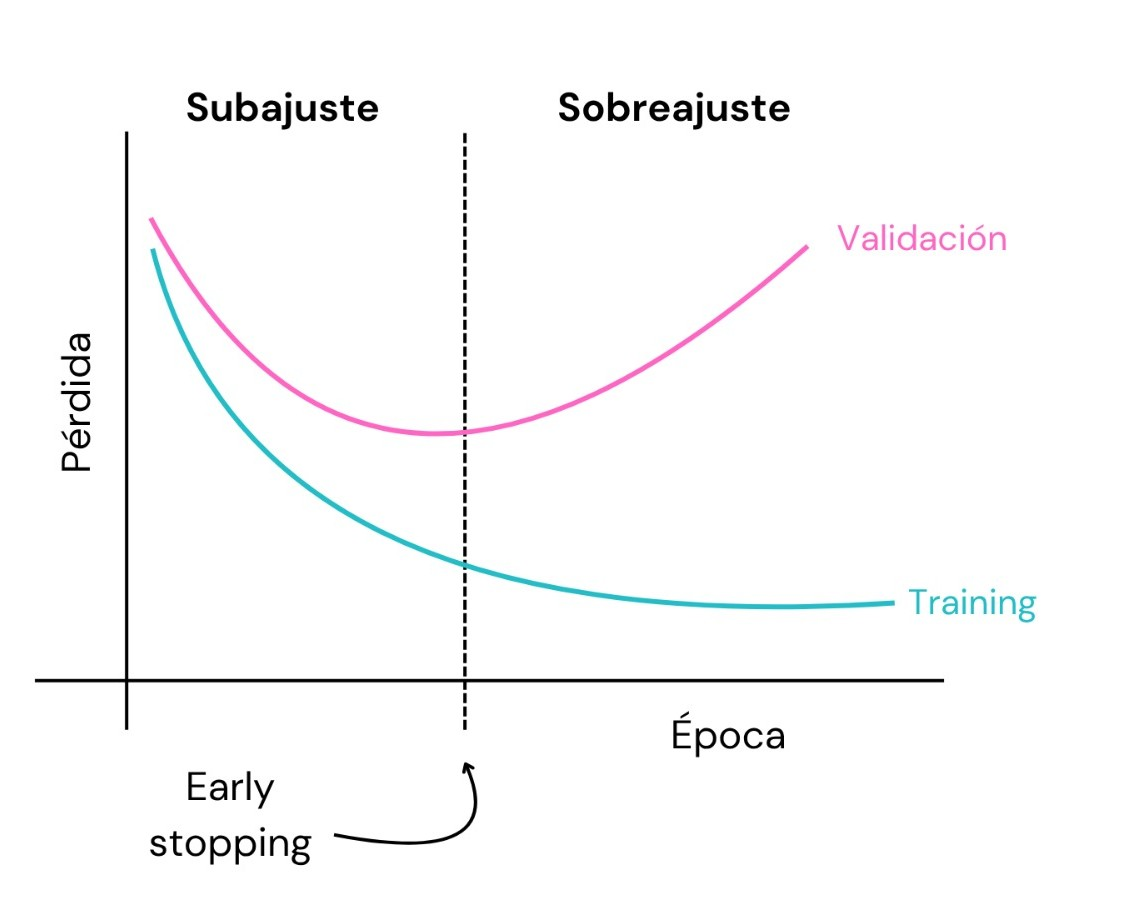
\includegraphics[width= 0.8 \textwidth]{img/early_stopping_grafico.jpeg}
    \caption{Representación gráfica del overfitting y del momento de actuación del early stopping, basada en la explicación gráfica de Holbrook \cite{holbrook2021overfitting}.}
    \label{fig:grafico_overfitting}
\end{figure}

\subsection{Data Augmentation}

El \textit{data augmentation} es una técnica fundamental en aprendizaje profundo que consiste en la generación de nuevas muestras de entrenamiento a partir de transformaciones sobre los datos originales. Estas transformaciones, como rotaciones aleatorias, cambios de escala y ajuste de contraste, permiten aumentar la diversidad del conjunto de datos sin necesidad de recopilar nuevas imágenes \cite{shorten2019da}.

Además, esta técnica contribuye a reducir el sobreajuste y mejorar la capacidad de generalización del modelo, permitiendo que las redes neuronales convolucionales puedan aprender representaciones más robustas incluso cuando se dispone de conjuntos de datos relativamente pequeños, como es el caso en este proyecto \cite{perez2017da}.

\subsection{Métricas de evaluación}
En tareas de segmentación de imágenes médicas, es crucial contar con métricas de evaluación que permitan cuantificar el rendimiento del modelo y garantizar que las predicciones realizadas sean útiles para su aplicación clínica.

\subsubsection{Matriz de confusión}
En el contexto del aprendizaje automático, la matriz de confusión es una herramienta fundamental para evaluar el rendimiento de un modelo de clasificación. Esto permite comparar las predicciones realizadas por el modelo con los valores reales, identificando aciertos y errores en la clasificación \cite{matrizconfusion}, como se ilustra en la Figura \ref{fig:matriz_confusion}.

\begin{figure}[h]
    \centering
    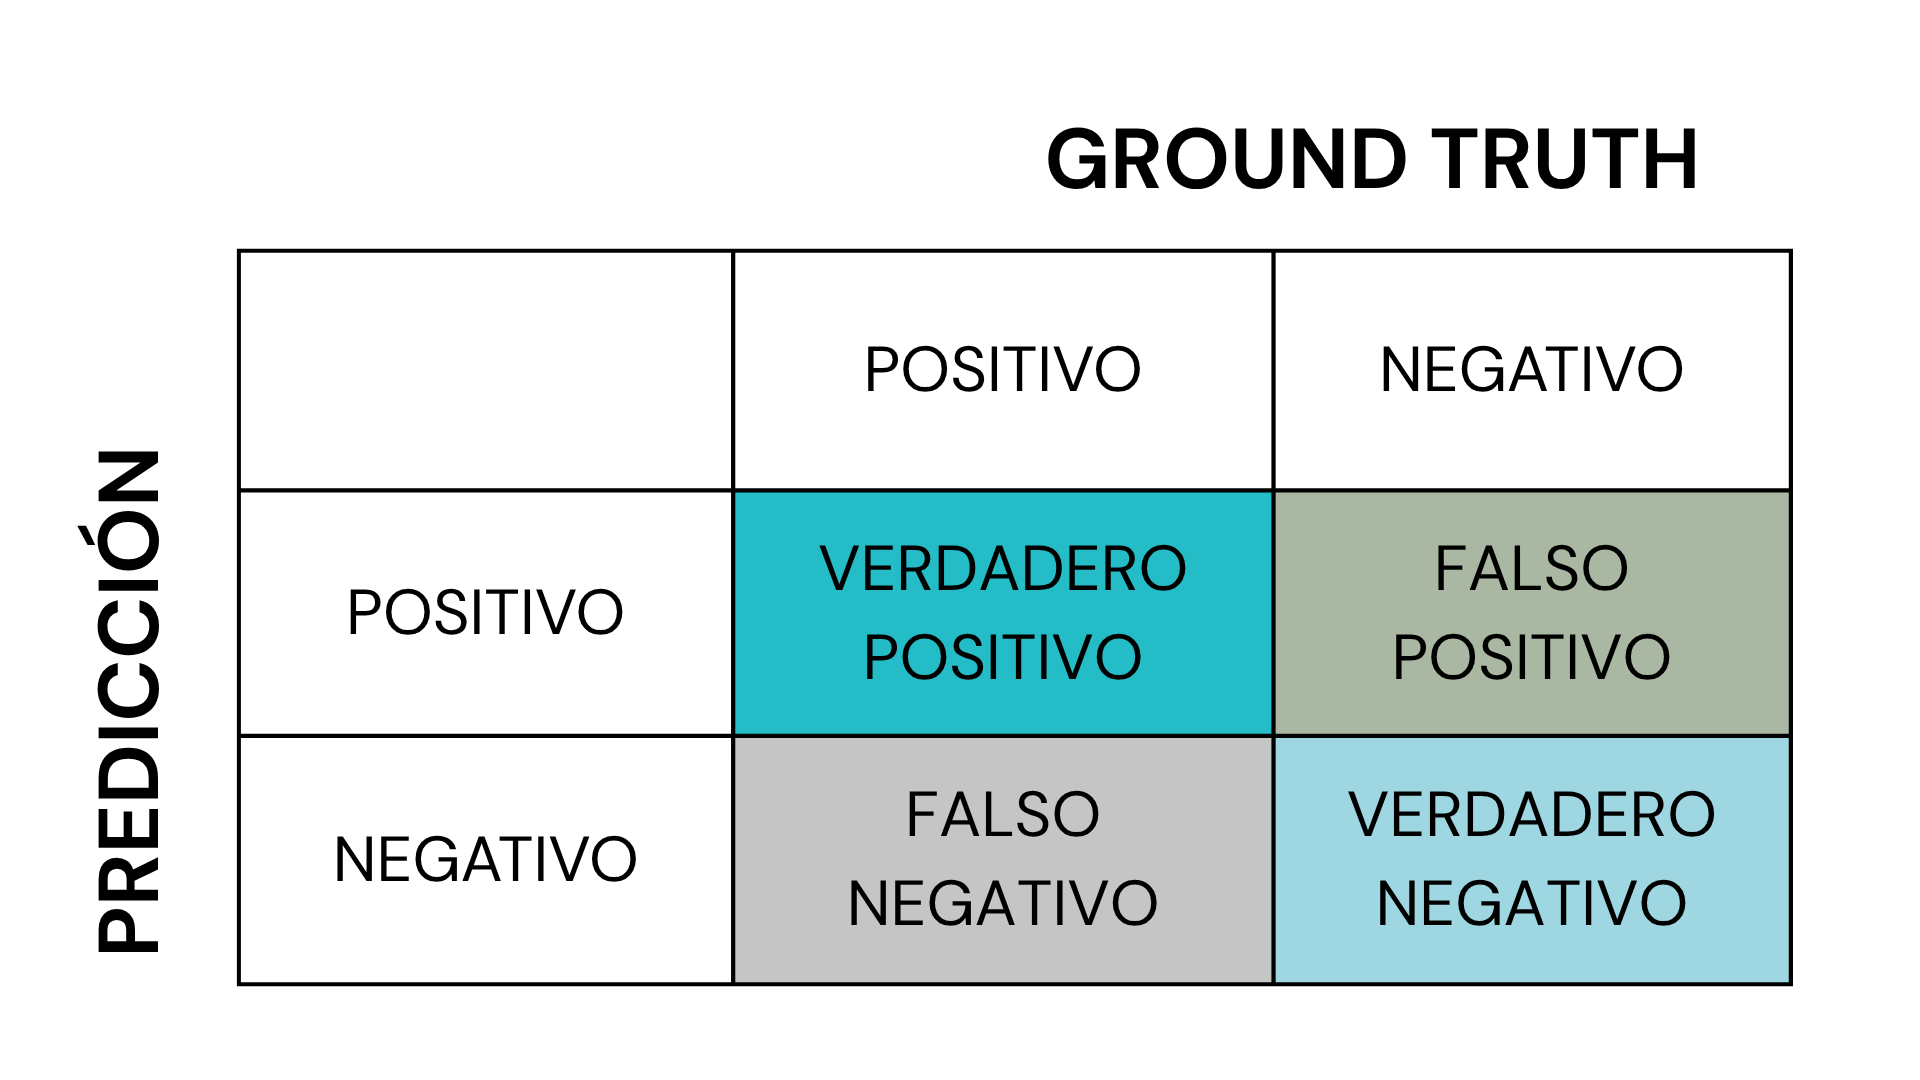
\includegraphics[width= 0.8 \textwidth]{img/matriz_confusion.png}
    \caption{Esquema ilustrativo de una matriz de confusión. Adaptado de \cite{matrizconfusionimage}}
    \label{fig:matriz_confusion}
\end{figure}
La matriz se organiza habitualmente con las clases reales en las filas y las claves predichas en las columnas. Entre los elementos que la componen destacan los verdaderos positivos (TP), que corresponden a las instancias correctamente clasificadas como positivas, y los falsos positivos (FP), que representan las instancias negativas que el modelo clasificó incorrectamente como positivas. Estos valores permiten calcular la precisión, una métrica clave para interpretar el comportamiento del modelo.

\subsubsection{Precisión}
También conocida como \textit{valor predictivo positivo}, se define como la proporción de TP entre el total de instancias clasificadas como positivas por el modelo, es decir, la suma de TP y FP \cite{Hossin2015precision}. Esta métrica evalúa la exactitud de las predicciones positivas realizadas por el modelo.
Matemáticamente, la precisión se expresa como: 
\begin{equation}
    \text{Precisión} = \frac{TP}{TP+FP}
\end{equation}
\subsubsection{Intersección sobre la Unión}
La métrica Intersección sobre la Unión o Intersection over Union (\texttt{IoU}) o Índice de Jaccard es ampliamente utilizada para evaluar la calidad de segmentaciones en tareas como la segmentación semántica, de instancias y panóptica. Esta métrica calcula la consistencia entre la máscara predicha por el modelo y la máscara de referencia (\textit{ground truth}), considerando todos los píxeles de las áreas segmentadas.

Matemáticamente, se define como:
\begin{equation}
    \text{\texttt{IoU}} = \frac{|P \cap G|}{|P \cup G|}
\end{equation}
donde \textit{P} representa la máscara predicha y \textit{G} la máscara de referencia. Se calculan los píxeles correctamente identificados como pertenecientes a una clase entre los píxeles etiquetados como pertenecientes a la clase de interés. La métrica toma valores entre 0 y 1, donde 1 indica una superposición perfecta. En este trabajo, se calcula un valor de \texttt{IoU} para cada clase segmentada y luego se obtiene la media de estos valores, que corresponde a la media global del rendimiento del modelo de segmentación. \cite{cheng2021iou}



